\documentclass[a4paper,12pt]{article}

\geometry{left=20mm,right=20mm,top=25mm,bottom=20mm} % задание полей текста
\usepackage{wrapfig}
%% Стиль колонтитулов
% \fancyhead[RO,LE]{\hyperlink{intro}{Содержание}} % Right odd,  Left even
\fancyhead[LO]{\@lecture}        % Right even, Left odd
\fancyhead[R]{}

\fancyfoot[RO,LE]{\thepage}         % Right odd,  Left even
\fancyfoot[RE,LO]{\CourseName}      % Right even, Left odd
\fancyfoot[C]{}
% Un~comment these to erase foot (and comment footrulewidth renewcommand)
%\fancyfoot{}
%\fancyhead[C]{-~\thepage~-}
\renewcommand{\footrulewidth}{0.4pt}
\usepackage{textcomp}

% Новая команда \lecture{№ лекции}{название}
% После этой команды весь текст до следующей такой же команды будет
% принадлежать конкретной лекции, имя которой будет в колонтитуле каждой страницы
\usepackage{xifthen}
\def\@lecture{}%
\newcommand{\lecture}[2]{
    \ifthenelse{\isempty{#2}}{%
        \def\@lecture{Лекция #1}%
    }{%
        \def\@lecture{Лекция #1: #2}%
    }%
    \section{\@lecture}
}

\def\@lecture{}%
\newcommand{\question}[2]{
    \ifthenelse{\isempty{#2}}{%
        \def\@lecture{Билет #1}%
    }{%
        \def\@lecture{Билет #1: #2}%
    }%
    \section{\@lecture}
}
% ------------ Text settings ------------
%%% Гиппер ссылки
\renewcommand{\linkcolor}{blue}
\renewcommand{\citecolor}{green}
\renewcommand{\filecolor}{magenta}
\renewcommand{\urlcolor}{NavyBlue}

\usepackage{multicol}	   % Для текста в нескольких колонках

% -----------  Images -----------
\graphicspath{{images/}{img/}{figures/}{fig/}}  % Путь к папкам с картинками
\newcommand{\figL}[3]{%      Для быстрой вставки картинок
    \begin{figure}[h!]
        \centering
        \includegraphics[width=#2\textwidth]{#1}
        \label{fig:#3}
    \end{figure}%
}
\newcommand{\fig}[2]{%    
    \begin{figure}[h!]
        \centering
        \includegraphics[width=#2\textwidth]{#1}
    \end{figure}%
}

% ----------- Math short-cats
\newcommand{\R}{\ensuremath{\mathbb{R}}}
\newcommand{\N}{\ensuremath{\mathbb{N}}}
\newcommand{\Cx}{\ensuremath{\mathbb{C}}}
\newcommand{\Z}{\ensuremath{\mathbb{Z}}}
\newcommand{\E}{\ensuremath{\mathbb{E}}}
\newcommand{\Q}{\ensuremath{\mathbb{Q}}}
\def\CB{\mathcal{B}}
\def\CC{\mathcal{C}}
\def\CE{\mathcal{E}}
\def\CR{\mathcal{R}}
\def\CA{\mathcal{A}}
% \def\CF{\mathcal{F}}
\def\CG{\mathcal{G}}
\def\CS{\mathcal{S}}
\def\CD{\mathcal{D}}
\def\CH{\mathcal{H}}
\def\CP{\mathcal{P}}
\def\CM{\mathcal{M}}
\def\FB{\mathfrak{B}}

% You can write your commands below
\usepackage{gensymb}
\usepackage{enumitem}
\usepackage{amsmath}
\newcommand{\F}{\ensuremath{\mathcal{F} }}
\newcommand{\Anu}{\ensuremath{\mathcal{A}_{\nu}}}
\DeclareMathOperator{\FDU}{FDU}

% ----------- Math and theorems -----------
\usepackage[many]{tcolorbox}
\usepackage{mdframed}
\usepackage[dvipsnames]{xcolor}

\newtheorem*{remark}      {Замечание}
\newtheorem*{next0}      {Следствие}
\newtheorem*{next1}      {Следствие 1}
\newtheorem*{next2}      {Следствие 2}
\theoremstyle{definition}
\newtheorem{lemma}{Лемма}[section]
\newtheorem{claim}[lemma]{Утверждение}
\newtheorem{theorem_}[lemma]{Теорема}
\newenvironment{theorem}%
{\begin{mdframed}[backgroundcolor=black!30!white!30]
        % \setlength{\topsep}{-\parskip}\setlength{\partopsep}{0pt}
        \begin{theorem_}}%
            {\end{theorem_}\end{mdframed}}

\theoremstyle{definition}
\newtheorem{definition}[lemma]{Определение}
\tcolorboxenvironment{definition}{
    enhanced,
    borderline={0.8pt}{0pt}{gray!70},
    borderline={0.4pt}{2pt}{black},
    boxrule=0.4pt,
    colback=pink!70!white!30,
    coltitle=black,
    sharp corners
}
\usepackage{ulem}
\newcommand{\mdef}[1]
{\! \textit{\uwave{\textcolor{red!10!black}{#1}}}}
% http://dkhramov.dp.ua/Comp.LatexCyrillicFonts#.XMrWLegzaUk


%https://tex.stackexchange.com/questions/223694/how-to-draw-a-text-box-with-shadow-borders-in-latex

\newtheorem{exercise_}[lemma]{Пример}
\newenvironment{exercise}%
{\begin{tcolorbox}[enhanced,width=\textwidth,center upper,drop fuzzy shadow southwest,
            colframe=red!50!black,colback=orange!100!yellow!50!white!30]
        \begin{exercise_}}%
            {\end{exercise_}\end{tcolorbox}}

\usepackage{dashrule}
\renewenvironment{proof}{\smallskip{\noindent\Large
        \color{red!50!black}\itshape$\lhd$ \normalsize Начало доказательства
        \hdashrule[0.5ex]{0.65\textwidth}{0.5mm}{3mm 3pt 1mm 2pt} }
    \small\itshape}{{\color{red!50!black}
            \hdashrule[0.5ex]{0.66\textwidth}{0.5mm}{3mm 3pt 1mm 2pt}
            \normalsize Конец доказательства \Large$\rhd$}}

\newenvironment{solution}{\smallskip{\noindent\Large
        \color{red!50!black}\itshape$\lhd$ \normalsize Начало решения
        \hdashrule[0.5ex]{0.75\textwidth}{0.5mm}{3mm 3pt 1mm 2pt} }
    \small}{{\color{red!50!black}
            \hdashrule[0.5ex]{0.75\textwidth}{0.5mm}{3mm 3pt 1mm 2pt}
            \normalsize\itshape Конец решения \Large$\rhd$}}

% Обводка кружочком множеств
\usepackage{tikz}
\usetikzlibrary{decorations.pathreplacing,shapes.misc,patterns}
\newcommand*\circled[1]{\tikz[baseline=(char.base)]{
        \node[shape=circle,draw,inner sep=2pt] (char) {#1};}}

\counterwithin*{equation}{section}

\usepackage{stackrel}
\newsavebox\MBox
\newcommand\Cline[2][red]{{\sbox\MBox{$#2$}%
            \rlap{\usebox\MBox}\color{#1}\rule[-1.2\dp\MBox]{\wd\MBox}{0.5pt}}}

%%% Всю шаблонную информацию можно менять тут
\newcommand{\FullCourseNameFirstPart}{\so{КРАТНЫЕ ИНТЕГРАЛЫ И}}
\newcommand{\FullCourseNameSecondPart}{\so{ТЕОРИЯ ПОЛЯ}}
\newcommand{\SchoolName}{ФПМИ}
\newcommand{\TrackName}{ПМИ, ИВТ, КТ, РАНХиГС}
\newcommand{\SemesterNumber}{III}
\newcommand{\LecturerInitials}{Лукашов Алексей Леонидович}
\newcommand{\AutherInitialsFirst}{Климов Ярослав}
\newcommand{\AutherInitialsSecond}{Ильдаров Адам}
\newcommand{\AutherInitialsThird}{Евдокимов Егор}
\newcommand{\VKLinkFirst}{https://vk.com/klimov_yaroslav}
\newcommand{\VKLinkSecond}{https://vk.com/adamildarov}
\newcommand{\VKLinkThird}{https://vk.com/ea_evdokimov}
\newcommand{\OverleafLink}{https://www.overleaf.com/read/thzfwhhyghfn}
\newcommand{\GithubLink}{https://github.com/MIPT-Group/Lectures_Tex_Club}

\newcommand{\CourseName}{Кратные интегралы и теория поля} %  Используется в преамбуле для создания названия предмета в верхнем контитуле   
\newcommand{\CourseDate}{2020}           %  Используется в преамбуле для создания даты в нижнем контитуле и в title_page

%\includeonly{lectures/lect05,lectures/lect06}  % Чтобы скомпилировать только часть лекций

\begin{document}
    %%% Всю шаблонную информацию можно менять тут
\newcommand{\FullCourseNameFirstPart}{\so{АРХИТЕКТУРА КОМПЬЮТЕРОВ И}}
\newcommand{\FullCourseNameSecondPart}{\so{ОПЕРАЦИОННЫЕ СИСТЕМЫ}}
\newcommand{\SchoolName}{ФПМИ}
\newcommand{\TrackName}{ПМИ}
\newcommand{\SemesterNumber}{III}
\newcommand{\LecturerInitials}{Яковлев Виктор Вадимович}
\newcommand{\AutherInitials}{Савелий Романов}
\newcommand{\VKLink}{https://vk.com/romanov_savelij}
\newcommand{\GithubLink}{https://github.com/MIPT-Group/Lectures_Tex_Club}

\begin{titlepage}
	\clearpage\thispagestyle{empty}
	\centering
	
	\textit{Федеральное государственное автономное учреждение \\
		высшего профессионального образования}
	\vspace{0.5ex}
	
	\textbf{Московский Физико-Технический Институт \\ КЛУБ ТЕХА ЛЕКЦИЙ}
	\vspace{20ex}
	
	\rule{\linewidth}{0.5mm}
	{\textbf{\FullCourseNameFirstPart}}
	\\
	{\textbf{\FullCourseNameSecondPart}}
	\rule{\linewidth}{0.5mm}
	
	\SemesterNumber\ СЕМЕСТР
	\\
	Физтех Школа: \textit{\SchoolName}
	\\
	Направление: \textit{\TrackName}
	\\
	Лектор: \textit{\LecturerInitials}
	\vspace{1ex}
	
	\begin{figure}[!ht]
		\centering
		
\includegraphics[width=0.6\textwidth, height=0.3\textheight]{logo_LTC}
		\label{fig:my_label}
	\end{figure}
\begin{flushright}
	\noindent
	Автор: \href{\VKLink}{\textit{\AutherInitials}}
	\\
	\href{\GithubLink}{\textit{Проект на github}} % Опционально, если хотите учавствовать в рейтинге
\end{flushright}
	
	\vfill
	\CourseDate\ года
	\pagebreak
	
\end{titlepage}
    \newpage
    \hypertarget{intro}{}
    \tableofcontents
    \newpage
    \setcounter{section}{7}
\section{Глава 8.}
\setcounter{subsection}{6}
\subsection{Принципы Литтлвуда}
Виды сходимостей:
\begin{enumerate}
    \item $f_n \rightarrow f \text{ п. в. (почти всюду) на } X \Leftrightarrow$ $$(\exists E\subset X,\  \mu (X\backslash E)=0)(\forall x \in E)(\forall \varepsilon > 0)(\exists N \in \N)(\forall n>N) \mid f_n(x)-f(x)\mid<\varepsilon$$
    \item $f_n \rightrightarrows f$ на $X$ (равномерно сходится) $\Leftrightarrow$ 
    $$(\forall \varepsilon > 0)(\exists N \in \N)(\forall n>N)(\forall x \in X) \mid f_n(x)-f(x)\mid<\varepsilon$$
    \item $f_n \Rightarrow f$ на $X$ (сходимость по мере)$\Leftrightarrow$
    $$(\forall \varepsilon > 0) \lim_{n\to\infty} \mu \{ x\in X: \mid f_n(x)-f(x)\mid \ \geqslant \varepsilon \} =0$$
    (не пишем, но помним: $X$ - измеримо по Лебегу, $f_n$ и $f$ - измеримы на множестве $X$)
\end{enumerate}
\begin{theorem}[Ф. Рисса]
    Если $f_n \Rightarrow f$ (сходится по мере) на $X$, то $\exists \{f_{n_k} \} ^\infty_{k=1}$ (подпоследовательность) $f_{n_k} \rightarrow f$ п. в. на $X$.
\end{theorem}
\begin{proof}
По определению сходимости по мере: $$(\forall i \in \N) \lim_{n\to\infty} \mu \{ x\in X: \mid f_n(x)-f(x)\mid \ \geqslant \frac{1}{i} \} =0$$ - меры этих множеств образуют бесконечно малую числовую последовательность. Тогда мы можем выбрать возрастающую подпоследовательность $$\{n_i\}^\infty_{i=1}:\  \mu \{ x\in X: \mid f_{n_i}(x)-f(x)\mid \ \geqslant \frac{1}{i} \} < 2^{-i}.$$
Последовательность $\{f_{n_i}\}^\infty_{i=1}$ и будет искомой, она будет сходится к $f$ почти всюду. Как это увидеть? Введем обозначения $$R_i:= \bigcup ^\infty_{k=i} \{x\in X:\ \mid f_{n_k}(x)-f(x)\mid \ \geqslant \frac{1}{k}\}$$. Что можно сказать о мере этих множеств?
\begin{equation}\label{1}
    \mu (R_i) \leqslant \sum_{k=i}^{\infty} \mu \{x\in X:\ \mid f_{n_k}(x)-f(x)\mid \ \geqslant \frac{1}{k}\} \leqslant \sum_{k=i}^{\infty} 2^{-k}=2^{-i+1}
\end{equation}
Также имеется такая цепочка включений $R_1\supset R_2 \supset \ldots \Rightarrow Q:=\bigcap\limits_{i=1}^\infty R_i$. Это пересечение, есть ни что иное, как $Q=\lim\limits_{i\to\infty}R_i$. Тогда $\mu(Q)=\lim\limits_{i\to\infty} \mu(R_i)=0$ (см \ref{1}).
\newpage Теперь мы хотим доказать что последовательность $\{f_{n_i}\}$ сходится к $f$ почти всюду. Положим в определении сходимости почти всюду $X\backslash E = Q$.
Тогда $$\forall x_0 \in X\backslash Q \Rightarrow x_0 \in \bigcup^\infty_{i=1}(X\backslash R_i) \Rightarrow \exists i_0, x_0 \in X\backslash R_{i_0} = \bigcap^\infty_{k=i_0} X\backslash \left\{x\in X:\ \mid f_{n_k}(x)-f(x)\mid \ \geqslant \frac{1}{k}\right\}$$
$x_0$ попадает в пересечение, это означает, что $(\forall k \geqslant i_0) \mid f_{n_k}(x_0)-f(x_0)\mid < \frac{1}{k}$, наконец: ${\lim\limits_{k\to\infty}f_{n_k}(x_0)=f(x_0)}$
\end{proof}

\begin{theorem}[Д. Ф. Егоров]
    Если $E$ измеримо по Лебегу, $f_n$ измеримы на $E$, конечны почти всюду на $E$ и $\lim\limits_{n\to\infty} f_n(x)=f(x)$ - равен почти всюду на $E$ и конечен почти всюду на $E$, то ${(\forall \varepsilon >0)(\exists E_{\varepsilon}\subset E,\ \mu (E\backslash E_{\varepsilon})<\varepsilon)\ f_n \rightrightarrows f}$ на $E_{\varepsilon}$
\end{theorem}
\begin{proof}
Обозначим через $E_m(\varepsilon):=\left\{x\in E:\ \mid f_m(x)-f(x)\mid\ \geqslant \varepsilon \right\}$

${\overline{\lim\limits_{m\to\infty}}E_m(\varepsilon) \subset E_0=\left\{x\in E:(f_n(x)\nrightarrow f(x)) \vee (f(x) \notin \R) \vee (\exists n\in \N:f_n(x)\notin \R) \right\},\ \mu(E_0)=0}$, где $E_0\text{ - множество, где все плохо. (Это включение доказывается в теореме 20 параграфа 5).}$

$\overline{\lim\limits_{m\to\infty}}E_m(\varepsilon) =\lim\limits_{n\to\infty}\sup\limits_{m\geqslant n} E_m(\varepsilon)=\bigcap\limits_{n=1}^{\infty}\bigcup\limits_{m=n}^{\infty}E_m(\varepsilon)$

$\lim\limits_{n\to\infty}\mu(\bigcup\limits_{m=n}^{\infty}E_m(\varepsilon))=0$

$(\forall i \in \N) {\lim\limits_{n\to\infty}} \mu(\bigcup\limits_{m=n}^{\infty}E_m(\frac{1}{i}))=0$

$\exists n_i\ \mu(\bigcup\limits_{m=n_i}^{\infty}E_m(\frac{1}{i}))<2^{-i}$

$\text{Если }x \in E \backslash {\bigcup\limits_{m=n_i}^\infty}E_m(\frac{1}{i}) \Rightarrow x \in \overset{\infty}{\underset{m=n_i}{\bigcap}}E\backslash E_m(\frac{1}{i})$

$(\forall \varepsilon >0)(\exists i_0) \sum\limits_{i=i_0}^{\infty}2^{-i}=2^{-i_0+1}<\varepsilon$

$E\backslash E_{\varepsilon}:=\bigcup\limits_{i=i_0}^{\infty}\bigcup\limits_{m=n_i}^{\infty}E_m(\frac{1}{i})$

$\mu(E\backslash E_{\varepsilon})\leqslant \sum\limits_{i=i_0}^{\infty}\mu(\bigcup\limits_{m=n_i}^{\infty}E_m(\frac{1}{i}))\leqslant \sum\limits_{i=i_0}^{\infty}2^{-i}<\varepsilon$

$(\forall x \in E_{\varepsilon}) \Rightarrow x \in \bigcap\limits_{i=i_0}^{\infty}\bigcap\limits_{m=n_i}^{\infty}E\backslash E_m (\frac{1}{i})$

$(\forall i \geqslant i_0)(\forall m \geqslant n_i) \mid f_m(x)-f(x) \mid < \frac{1}{i}$

$(\forall \delta > 0)(\exists N)(\forall m \geqslant N)(\forall x \in E \backslash E_{\varepsilon}) \mid f_m(x)-f(x) \mid < \delta$ - это и означает равномерную сходимость на множесте $E_{\varepsilon}$
\end{proof}
\newpage
\begin{theorem}[Структура открытых множеств в $\mathbb{R}^1$]
    Если $G \subset \R^1$ - открытое, то оно является дизъюнктным объединением конечного или счетного числа интервалов $G=\bigsqcup\limits_{i=1}^{\infty}(a_i, b_i)$
\end{theorem}
\begin{proof}
Введем между точками множества $G$ отношение эквивалентности: $x, y\in G$ называются эквивалентными $x\sim y$, если интервал с концами $x, y\ ((x, y)\text{ или }(y,x)) \subset G$. $G$ разбивается на дизъюнктное объединение классов эквивалентности. Докажем, что класс - интервал. Пусть $K$ - класс, обозначим ${a:=\inf\limits_{x \in K}x,\ b:=\sup\limits_{x\in K}x}$. Пусть $c \in (a,b) \Rightarrow {\exists \alpha \in K \cap (a, c),\ \beta \in K \cap (c, b) \Rightarrow  (\alpha, \beta)\subset K  \Rightarrow c \in K} \Rightarrow (a,b) \subset K$.

Теперь, чтобы доказать, что $K$ именно интервал, необходимо доказать, что концы не попадают. Пусть $a \in K \subset G$, где $G$ - открытое, тогда $(\exists d >0)(a-d, a+d)\subset G \Rightarrow {a-\frac{d}{2} \sim a} \Rightarrow a-\frac{d}{2} \in K$. Это является противоречием с тем, что $a$ точная нижняя грань. Итого $(a, b)=K$
\end{proof}

Принципы Литтлвуда:
\begin{enumerate}
    \item Каждое измеримое множество --- это приблизительно объединение конечного числа интервалов.
    \item Сходимость почти всюду --- это приблизительно равномерная сходимость.
    \item Измеримые функции приблизительно непрерывны.
\end{enumerate}
\begin{theorem}[Н. Н. Лузин]
	Если $f$ измеримая и почти всюду конечная на $[a, b]$, то ${(\forall \varepsilon >0)(\exists E_{\varepsilon},\  \mu([a, b] \backslash E_{\varepsilon})<\varepsilon) (\exists \varphi \in C[a,b](\text{непрерывная}))\text{, такая что }(\forall x \in E_{\varepsilon}) \ f(x)=\varphi(x)}$
\end{theorem}
\begin{proof}
Пусть $|f(x)|\leqslant C$. Теорема 19 \textsection 5  утверждает, что можно подобрать последовательность ступенчатых функций, которая равномерно сходится к $f(x)$, т. е. существует $h_n(x) \rightrightarrows f(x)$. Так как $f(x)$ ограничена, то все $h_n(x)$ имеют лишь конечное множество значений, то есть $h_n$ постоянна на множествах $I_{n, 1}, \ldots, I_{n, k_n}$, где $k_n$ - количество различных значений. Эти множества измеримы по Лебегу. И также $\bigsqcup\limits_{k=1}^{k_n} I_{n, k}=[a,b]$. Из первого принципа Литтлвуда $$\forall k=1, \ldots, k_n\ \exists \text{ замкнутое множество } F_{n,k} \subset I_{n,k} \text{ т. ч. } \mu(I_{n,k}\backslash F_{n,k})<\dfrac{\varepsilon \cdot 2^{-n-1}}{k_n}.$$ Также из того, что $h_n(x) \rightrightarrows f(x)$ на всем $[a,b]$, следует, что сходится на любом подмножестве: $h_m(x) \rightrightarrows f(x)$ на $\bigcup\limits_{k=1}^{k_n} F_{n,k}=: K_n$. Положим $\bigcap\limits_{n=1}^{\infty} K_n =: E_{\varepsilon}$. Рассмотрим $\mu ([a,b] \backslash E_{\varepsilon}) = \mu(\bigcup\limits_{n=1}^{\infty}([a,b] \backslash K_n)) \leqslant \sum\limits_{n=1}^{\infty}\mu([a,b]\backslash K_n) = \sum\limits_{n=1}^{\infty} \sum\limits_{k=1}^{K_n}\mu(I_{n,k}\backslash F_{n,k}) \leqslant \sum\limits_{n=1}^{\infty}\varepsilon\cdot 2^{-n-1}=\dfrac{\varepsilon}{2}<\varepsilon$.

$h_n \rightrightarrows f$ на $E_{\varepsilon}$, заметим $h_n \text{ на } K_n$ непрерывна. Почему это так? $K_n$ - это конечное объединение замкнутых множеств, и на каждом из этих множеств функция постоянная. Непрерывность означает $\forall x_0 \in K_n, \{x_m\}\subset K_n,$ ${ \lim\limits_{m\to\infty}x_m = x_0}, \lim\limits_{m\to\infty}h_n(x_m)=h_n(x_0).$ Пусть $x_0 \in K_n \Rightarrow \exists !\ k : x_0 \in F_{n, k} \Rightarrow \exists\ M\  \forall m > M\ \ x_m \in F_{n,k}$, и еще $h_n$ постоянная на $F_{n,k} \Rightarrow h_n(x_m)=h_n(x_0)$, что доказывает непрерывность $h_n$ на $K_n$. Значит $h_n$ непрерывно на $E_{\varepsilon}$. Мы имеем последовательность нерперывных на замкнутом множестве функций, такую что на этом множестве она равномерно сходится, тогда по следствию из теоремы о предельном переходе в равномерно сходящихся последовательностях $h_n \rightrightarrows$ к непрерывной на $E_{\varepsilon}$ функции. Для завершения доказательства осталось установить, что функцию непрерывную на замкнутом подмножестве $[a,b]$ можем продолжить до непрерывной на все отрезке $[a,b]$. Введем $\alpha := \inf\limits_{x\in E_\varepsilon}x,\ \beta := \sup\limits_{x\in E_\varepsilon}x$. В силу замкнутости $\alpha, \beta \in E_\varepsilon$.
\begin{equation*}
\varphi (x) := \begin{cases}
f(x),\ x\in E_\varepsilon\\
f(\alpha),\ x \in [a,\alpha)\\
f(\beta),\ x \in (\beta, b]\\
\text{линейна на каждом }(\lambda_i, \mu_i) (\text{с непрерывностью в }\lambda_i, \mu_i),
\end{cases}
\end{equation*}
где $[\alpha, \beta]\backslash E_\varepsilon = (\alpha, \beta)\backslash E_\varepsilon = (\alpha, \beta)\cap(\R \backslash E_\varepsilon)=\bigsqcup\limits_{i=1}^\infty(\lambda_i, \mu_i)$. Осталось доказать, что $\varphi (x)$ непрерывная на $[a,b].$

Возьмем произвольное $x_0 \in [a,b], \{x_m\}\subset [a,b], \lim\limits_{m\to\infty}x_m=x_0 \overset{?}{\Rightarrow} \lim\limits_{m\to\infty}\varphi (x_m)=\varphi (x_0)$. В каких случаях это не тривиально? 
\begin{equation*}
\begin{cases}
 x_0 \in E_\varepsilon\text{ - не является правым концом } (\lambda_i, \mu_i) \\
 x_1 < x_2 < \ldots \notin E_\varepsilon
\end{cases}
\end{equation*}
Тогда $x1,\ldots, x_{n_1} \in (\lambda_1, \mu_1),\newline x_{n_1+1}, \ldots, x_{n_2} \in (\lambda_2, \mu_2)$ и т. д. Но значения $\varphi$ в этих точках находится между $(\varphi(\lambda_i),\varphi( \mu_i)).$ Так как $\{x_m\}$ стремится к $x_0$, то соответствующие $\lambda$ и $\mu$ тоже стремятся к $x_0$, и по теореме о трех силовиках $\varphi(x)$ стремится к $\varphi(x_0)$

Теперь докажем теорему без предположения об ограниченности $f(x)$. Рассмотрим множества $A_k:=\{x\in [a,b]: |f(x)|>k \}$. Из такого определения следует, что $A_1 \supset A_2 \supset \ldots$ Тогда $\lim\limits_{k\to\infty} A_k=\bigcap\limits_{k=1}^{\infty}A_k={\{x\in [a,b]: | f(x) | =+\infty\},}\ \mu(\bigcap\limits_{k=1}^{\infty}A_k=0) \Rightarrow \lim\limits_{k\to\infty}\mu (A_k)=0$. Раз предел некоторой числовой последовательности равен 0, то $(\forall \varepsilon >0)(\exists k_0)\ \mu (A_k)<\dfrac{\varepsilon}{2}$. Положим 
\begin{equation*}
    g(x):=\begin{cases}
    f(x), x\in [a,b]\backslash A_{k_0}\\
    k_0, x \in A_{k_0}
    \end{cases}
\end{equation*}
Тогда $\mu (x\in [a,b]:f(x)=g(x))=(b-a)-\mu(A_{k_0})$. Функция $g(x)$ измеримая и ограниченная, значит по-доказанному мы можем выбрать $E_\varepsilon$ и функцию $\varphi(x)$ такие, что ${\mu ([a,b]\backslash E\varepsilon)<\dfrac{\varepsilon}{2} }$ $(\forall x \in E_\varepsilon)\ \varphi(x)=g(x) \Rightarrow \varphi(x) = f(x)\  \forall x \in E_\varepsilon \cap ([a,b]\backslash A_{k_0})$. Значит $\mu([a,b]\backslash(E_\varepsilon\cap([a,b]\backslash A_{k_0})))=$ $\mu(([a,b]\backslash E\varepsilon)\cup A_{k_0})\leqslant \mu([a,b]\backslash E_\varepsilon)+\mu(a_{k_0})<\varepsilon.$

\end{proof}
    \newpage
   	\begin{flushright}
    \textit{Лекция 2 (от 08.09)}
\end{flushright}
\section{$\S 3.$ Дифференцирование}
Пусть $z_0 \in \CC$, $B_r(z_0)$ и $f: B_r(z_0) \mapsto \CC$
\Def
Пусть $f: B_r(z_0) \mapsto \CC$. Если
\begin{equation}\label{(3.1)}
    \exists \dst \lim_{z \mapsto z_0} \frac{f(z)-f(z_0)}{z-z_0}
\end{equation}
то он называется \textbf{производной функции $f$ в точке $z_0$} (записывается
$f'(z_0)$).
\\
Можем расписать предел:
\begin{equation}\label{(3.2)}
    \forall \varepsilon > 0 \exists \delta(\varepsilon)>0: \ z \in B_\delta(z_0), \ \left| \frac{f(z) - f(z_0)}{z-z_0} - f'(z_0) \right| < \varepsilon
\end{equation}
\begin{equation}\label{(3.3)}
    f(z) = f(z_0) + f'(z_0)(z-z_0) + \alpha(z-z_0)
\end{equation}
\begin{equation}\label{(3.4)}
    \lim_{z \to z_0}\frac{\alpha(z-z_0)}{z-z_0} = 0
\end{equation}
\begin{align*}
  & f(z_0) = u(x,ym) + iv(x,y)
\end{align*}
\Def
Говорят, что $f: B_r(z_) \mapsto \CC$ \textbf{дифференцируема в точке $z_0$},
если
\begin{equation}\label{(3.5)}
    \exists A \in \CC: \ f(z) = f(z_0)+A(z-z_0)+o(z-z_0)
\end{equation}
\lemma
$f: B_r(z_0) \mapsto \CC$ дифференцируема в $z_0$ $\Leftrightarrow$ $\exists
f'(z_0)$, $A = f'(z_0)$
\pr
Очевидно.
\\
Обозначим: $\Delta x = x-x_0$, $\Delta y = y - y_0$, $\Delta z = z-z_0 = \Delta
x + i \Delta y$, $\Delta u = u(x,y)-u(x_0,y_0)$, $\Delta v = v(x,y)-v(x_0,y_0)$,
$\Delta f = f(x,y)-f(x_0,y_0) = \Delta u + i \Delta v$.
\theorem
$f: B_r(z_0) \mapsto \CC$ дифференцируема в $z_0$ т огда и только тогда, когда
\begin{itemize}
    \item $u(x,y)$, $v(x,y)$ дифференцируемы в $(x_0,y_0)$ (в $\RR^2$)
    \item выполняется условие Коши-Римана (УКР):
    \begin{equation}\label{(3.6)}
        \left\{ \begin{matrix}
                \dst \frac{\partial u}{\partial x} = \dst \frac{\partial v}{\partial y} \\
                \dst \frac{\partial v}{\partial x} = - \dst \frac{\partial u}{\partial y}
            \end{matrix} \right.
    \end{equation}
\end{itemize}
При этом
\begin{equation}\label{(3.7)}
    f'(z_0) = \frac{\partial u}{\partial x}(x_0,y_0) + i\frac{\partial v}{\partial x}(x_0,y_0) = \frac{\partial v}{\partial y}(x_0,y_0) - i\frac{\partial u}{\partial y}(x_0,y_0)
\end{equation}
\pr
Докажем в обе стороны.
\begin{itemize}
    \item Необходимость.
    \begin{align*}
      & \exists f'(z_0) = a+ib = A \in \CC
    \end{align*}
    Значит, по определению дифференцируемости
    \begin{align*}
      & \Delta f = A \Delta z + \alpha(\Delta z); \ \alpha(\Delta z) = \alpha_1(\Delta x, \Delta y) + \alpha_2(\Delta x, \Delta y)
    \end{align*}
    \begin{align*}
      & \left\{ \begin{matrix}
              \Delta u = a \Delta x - b \Delta y + \alpha_1(\Delta x, \Delta y) \\
              \Delta v = b \Delta x + a \Delta y + \alpha_2(\Delta x, \Delta y)
          \end{matrix} \right.
    \end{align*}
    \begin{align*}
      & \left| \alpha_1 \right| \leq \left| \alpha \right|, \ \left| \alpha_2 \right| \leq \left| \alpha \right|
    \end{align*}
    \begin{align*}
      & \lim_{(\Delta x; \Delta y) \to (0;0)}\left( \frac{\left| \alpha_1(\Delta x, \Delta y) \right|}{\sqrt{\left( \Delta x \right)^2 + \left( \Delta y \right)^2}} \right) \leq \lim_{\Delta z \to 0}\left( \frac{\left| \alpha(\Delta z) \right|}{\left| \Delta z \right|} \right) = 0
    \end{align*}
    Значит, $u$ дифференцируема, причем $\dst \frac{\partial u}{\partial x} =
    a$, $\dst \frac{\partial u}{\partial y} = -b$.
    \\
    Аналогично для $v$, причем $\dst \frac{\partial v}{\partial x} = b$, $\dst
    \frac{\partial v}{\partial y} = a$.
    \\
    Видим выполнимость УКР.
    \\
    Выполнимость \eqref{(3.7)} очевидна.
    \item Достаточность.
    \\
    Пусть $u$, $v$ дифференцируемы в $(x_0,y_0)$ и выполняется УКР. Тогда
    \begin{align*}
      & \Delta f = \Delta u + i \Delta v = \frac{\partial u}{\partial x} \Delta x + \frac{\partial u}{\partial y} \Delta y + \alpha_1(\Delta x, \Delta y) + i \left( \frac{\partial v}{\partial x} \Delta x + \frac{\partial v}{\partial y} \Delta y + \alpha_2(\Delta x, \Delta y)\right) = \\
      & \frac{\partial u}{\partial x} \Delta x - \frac{\partial v}{\partial x} \Delta y + \alpha_1(\Delta x, \Delta y) + i \left( \frac{\partial v}{\partial x} \Delta x + \frac{\partial u}{\partial x} \Delta y + \alpha_2(\Delta x, \Delta y)\right) = \left( \frac{\partial u}{\partial x} + i \frac{\partial v}{\partial x}\right)\cdot \\
      & \cdot \left( \Delta x + i \Delta y \right)+ \alpha_1(\Delta x, \Delta y) + i \alpha_2(\Delta x, \Delta y)
    \end{align*}
    Значит,
    \begin{align*}
      & \exists f'(z_0) = \frac{\partial u}{\partial x} + i \frac{\partial v}{\partial x}
    \end{align*}
\end{itemize}
\Example
\begin{align*}
  & w = z^2
\end{align*}
\begin{itemize}
    \item[I] Найдем производную по определению.
    \begin{align*}
      & \frac{\Delta w}{\Delta z} = \frac{\left( z_0-\Delta z \right)^2 - z_0^2}{\Delta z} = \frac{2z_0\Delta z + \left( \Delta z \right)^2}{\Delta z} = 2z_0 \Delta z \us{\Delta z \to 0}{\to} 2z_0
    \end{align*}
    \item[II] Найдем производную с использованием теоремы.
    \begin{align*}
      & z^2 = x^2-y^2+2ixy \Rightarrow u = x^2-y^2, \ v = 2xy
    \end{align*}
    \begin{align*}
      & u_x = 2x = v_y; \ u_y = -2y = - v_x
    \end{align*}
    Видим выполнимость УКР, поэтому
    \begin{align*}
      & w' = u_x+iv_x = 2x + 2iy = 2z
    \end{align*}
\end{itemize}
\Example
\begin{align*}
  & w = \left| z \right|^2
\end{align*}
\begin{align*}
  & \left| z \right|^2 = x^2+y^2 \Rightarrow u = x^2+y^2, \ v = 0
\end{align*}
\begin{align*}
  & u_x = 2x \neq 0 = v_y; \ u_y = 2y \neq 0 = - v_x
\end{align*}
(за исключением точки $(0;0)$). Видим выполнение УКР только в точке $(0;0)$, а
значит, и функция дифференцируема только в этой точке (с производной, равной
$0$).
\Example
\begin{align*}
  & w = \ol{z}
\end{align*}
\begin{align*}
  & \ol{z} = x - iy \Rightarrow u = x, \ v = -y
\end{align*}
\begin{align*}
  & u_x = 1 \neq -1 = v_y; \ u_y = 0 = - v_x
\end{align*}
Видим, что УКР не выполняется ни в одной точке $\CC$, а значит, функция нигде не
дифференцируема.
\prop
Если $f(z)$, $g(z)$ дифференцируемы, то:
\begin{itemize}
    \item дифференцируема и сумма:
    \begin{align*}
      & \left( f+g \right)' = f'+g'
    \end{align*}
    \item дифференцируемо и произведение:
    \begin{align*}
      & \left( fg \right)' = f'g+fg'
    \end{align*}
    \item дифференцируемо и частное (когда $g(z) \neq 0$):
    \begin{align*}
      & \left( \frac{f}{g} \right)' = \frac{f'g+fg'}{g^2}
    \end{align*}
\end{itemize}
\pr
Доказательства легко провести через УКР с использованием действительного
анализа.
\section{$\S 4.$ Регулярные и гармонические функции}

   	\newpage
   	\begin{flushright}
    \textit{Лекция 3 (от 14.09)}
\end{flushright}
\section{$\S 5.$ Теорема об обратной функции}
\theorem
Пусть $f: G \mapsto H \subseteq \CC$, $g: H \mapsto \CC$ регулярны.
Тогда $\xi(z) = g(f(z)): G \mapsto \CC$ также регулярна, причем $\xi'(z) =
g'(f(z))f'(z) \forall z \in G$.
\pr
$$z_0 \in G, \ w_0 = f(z_0) \in H$$
$$\Delta f = f(z_0)\Delta z + o(\Delta z)$$
$$\Delta g = g'(w_0) \Delta w + 0(\Delta w)$$
Пусть $\Delta w = \Delta f$
$$\frac{\Delta \xi}{\Delta z} = g'(w_0) \frac{\Delta f}{\Delta z} +
\frac{o(\Delta f)}{\Delta f} \cdot \frac{\Delta f}{\Delta z} \rightarrow
g'(w_0)f'(z_0) + 0$$
\section{$\S 6.$ Интегрирование}
   	\begin{flushright}
    \textit{Лекция 4 (от 15.09)}
\end{flushright}

\textbf{Кривая} $\gamma$~--- класс эквивалентных параметризаций $z(t) = x(t) +
iy(t), \ t \in \left[ t_0; t_1 \right]$
\\
\textbf{Параметризации эквивалентны}, если существует монотонная возрастающая
функция $\psi(\tau) = t$, сохраняющая направление.
\\
\textbf{Гладкая кривая (ГК)}~--- такая кривая $\gamma$, что существует параметризация
$z(t) = x(t) + iy(t)$, $x \in C^1 \left( \left[ t_0; t_1 \right] \right)$, $y
\in C^1 \left( \left[ t_0; t_1 \right] \right)$, $\forall t \in \left[ t_0; t_1
\right] \ z'(t) \neq 0$.
\\
\textbf{Замкнутая ГК (ЗГК)}~--- такая ГК, что $z(t_0) = z(t_1)$, $z'(t_0+0) =
z'(t_1-0)$.
\\
\textbf{Кусочно гладкая кривая (КГК)}~--- такая непрерывная кривая $\gamma$, что
$\exists t_0 = \theta_0 < \theta_1 < \dots < \theta_{n-1} < \theta_n = t_1$, что
$\forall k \ \gamma_k: \ z(t), \ t \in [\theta_{k-1}, \theta_k]$ есть ГК.
\\
\textbf{Разбиение} отрезка $\left[ t_0, t_1 \right]$: $\lambda = \{t_0 = \tau_0
< \tau_1 < \dots < \tau_{m_\lambda} = t_1\}$.
\\
\textbf{Мелкость (диаметр)} разбиения $\lambda$ $\left| \lambda \right| = \dst
\max_{k \{1, \dots, m_\lambda\}}\left| \tau_k - \tau_{k-1} \right|$.
\Def Пусть $f: \gamma \mapsto \CC$ непрерывна на КГК $\gamma$. Пусть
$\lambda$~--- разбиение $\left[ t_0, t_1 \right]$ для $\gamma: \ z(t)$~---
кусочно гладкой. Пусть $z(t_k) = z_k, \ k \in \{0, \dots, m_\lambda\}$, $\zeta_k
\in$
\[\sigma(\lambda) = \sum_{k = 1}^{m_{\lambda}} f(\zeta_k) \Delta z_k\]
$\Delta z_k = z_k - z_{k-1}$~--- \textbf{интегральная сумма};
\\
если $\exists \lim
\sigma(\lambda) \forall \zeta_k, \ \left| \lambda \right| \to 0$, то этот предел
называется \textbf{интегралом Римана от $f$ по $\gamma$} и записывается как
\begin{equation} \label{(6.1)}
  \int_{\gamma}f(z) dz
\end{equation}
\theorem
Если условия определения интеграла выполняются, то он существует и справедливо:
\begin{equation} \label{(6.2)}
    \int_{\gamma}f(z)dz = \int_{\gamma}\left( u dx - v dy \right) + i \int_\gamma \left( v dx + u dy \right)
    \end{equation}
\pr
\begin{align*}
  & \sigma(\lambda) = \sum_{k = 1}^{m_\lambda}\left( u(\xi_k, \eta_k) + iv(\xi_k, eta_k) \right)\left( \Delta x_k + i \Delta y_k \right) = \sum_{k = 1}^{m_\lambda}\left( u(\xi_k, \eta_k) \Delta x_k - v(\xi_k, \eta_k) \Delta y_k\right) + \\
  & + \left( v(\xi_k, \eta_k) \Delta x_k + u(x_k, y_k) \Delta y_k\right) = \sigma_1(\lambda) + \sigma_2(\lambda) \to \int_{\gamma}\left( u dx - v dy \right) + i \int_\gamma \left( v dx + u dy \right)
\end{align*}
\corollary
Если условия определения интеграла выполняются, то верно:
\begin{equation} \label{(6.3)}
  \int_\gamma f(z) dz = \int_{t_0}^{t_1}f(z(t))z'(t)dt
\end{equation}
\begin{equation} \label{(6.4)}
  \gamma: z(t), \ \int_{t_0}^{t_1}\left( P(t) + iQ(t) \right) dt = \int_{t_0}^{t_1}P(t)dt + i \int_{t_0}^{t_1}Q(t)dt
\end{equation}
\pr
Из \eqref{(6.2)} и свойств криволинейных интегралов II рода
\begin{align*}
  &\int_{\gamma}P(x,y) dx + Q(x,y)dy = \int_{t_0}^{t_1} \left( P(x(t), y(t)x'(t) + Q(x(t), y(t))y'(t) \right) dt
\end{align*}
\underline{\textbf{Общие свойства интеграла}}
\begin{enumerate}
    \item Линейность:
    \begin{align*}
      &\int_{\gamma}\left(\lambda f(z) + \mu g(z)\right) dz = \lambda\int_{\gamma}f(z) dz + \mu \int_\gamma g(z) dz
    \end{align*}
    \item Аддитивность вдоль кривой: если $\gamma = \gamma_1 \cup \gamma_2$
    (общая точка~--- только конец), то
    \begin{align*}
      &\int_{\gamma}f(z) dz = \int_{\gamma_1}f(z) dz \int_{\gamma_2} f(z) dz
    \end{align*}
    \item Изменение знака при смене направления: если $\gamma^{-1}$~---
    кривая, совпадающая во всех точках с $\gamma$, но противоположно
    направленная, то
    \begin{align*}
      &\int_{\gamma^{-1}}f(z) dz = - \int_{\gamma}f(z) dz
    \end{align*}
    \item Инвариантность относительно замены параметра.
    \item Выполняется неравенство:
    \begin{equation} \label{(6.5)}
      \left| \int_\gamma f(z) dz \right| \leq \int_{\gamma}\left| f(z) \right| \cdot \left| dt \right| = \int_{t_0}^{t_1} \left| f(z(t)) \right| \sqrt{(x'(t))^2 + (y'(t))^2}dt
    \end{equation}
    \pr
    Из \eqref{(6.3)}:
    \begin{equation} \label{(6.6)}
      \left| \sigma(\lambda) \right| \leq \sum_{k = 1}^{m_\lambda}\left| f(\zeta) \right| \cdot \left| \Delta z_k \right|
    \end{equation}
\end{enumerate}
\example
\begin{align*}
  &J_k = \int_{\gamma: \left| z-a \right| = r} (z-a)^k dz, \ k \in \ZZ
\end{align*}
Параметр: $z(t_ = a+re^{it}), \ t \in [0;2\pi]$
\\
$dz(t) = rie^{it}dt$
\begin{align*}
  &J_k = \int_{0}^{2\pi} r^ke^{ikt}rie^{it}dt = r^{k+1}i\int_{0}^{2\pi}e^{i(k+1)t} dt
\end{align*}
\begin{align*}
  &J_{-1} = 2 \pi i
\end{align*}
\begin{align*}
  &J_k = r^{k+1}i\int_{0}^{2\pi} \left( \cos(k+1)t + i \sin(k+1)t \right) dt = 0, \ k \neq -1
\end{align*}
\example
\begin{align*}
  &J_1 = \int_{\gamma} dz, \ J_2 = \int_{\gamma}z dz
\end{align*}
$\gamma: z(t)$, и согласно \eqref{(6.3)}
\begin{align*}
  &J_1 = \int_{t_0}^{t_1} z'(t)dt = z(t_1) - z(t_0)
\end{align*}
\begin{align*}
  &J_2 = \int_{t_0}^{t_1} z(t)z'(t)dt = \frac{1}{2}\int_{t_0}^{t_1}\frac{d}{dt}\left( z^2(t) \right)dt = \frac{1}{2}\left( z^2(t_1) - z^2(t_0) \right)
\end{align*}
\theorem
Пусть $f_n: G \mapsto \CC$ непрерывна на $G$ $\forall n \in \NN$, $\gamma$~---
КГК, $\gamma \subseteq G$.
\\
Пусть $\dst \sum_{n=1}^{\infty}f_n(z) \underset{\gamma}{\rightrightarrows} \rightarrow_{\gamma} S(z)
\forall z \in \gamma$.
Тогда $S(z)$ непрерывна на $\gamma$ и выполняется
\begin{equation} \label{(6.7)}
  \int_{\gamma}S(z) dz = \sum_{n=1}^{\infty}\int_{\gamma}f_n(z)dz
\end{equation}
\pr
Ряд сходится равномерно на $\gamma$
\\
$$\Updownarrow$$
\begin{equation} \label{(6.8)}
  \forall \varepsilon > 0 \exists N(\varepsilon): \forall N\geq N(\varepsilon) \ \underset{z \in \gamma}{\sup} \left| S(z) - \sum_{n = 1}^{N} \right| = \underset{z \in \gamma}{\sup} S_N(z) \leq \varepsilon
\end{equation}
\begin{align*}
  &\exists \delta > 0: \ \forall z_0 \in \gamma, \ z \in \gamma, \ \left| z - z_0 \right| < \delta: \ \left| S(z) = S(z_0) \right| \leq \left| S(z) - S_N(z) \right| +  \left| S_N(z) - \right. \\
  &\left. - S_N(z_0) \right| + \left| S_N(z_0) - S(z_0) \right| \leq \left| S_N(z) - S_N(z_0) \right| + 2 \varepsilon \leq 3 \varepsilon
\end{align*}
$$\Downarrow$$
$$S(z) \rightarrow S(z_0)$$
$$\Downarrow$$
$$\exists \int_{\gamma}S(z)dz$$
\begin{align*}
  &\forall N \geq N(\varepsilon) \ \left| \int_{\gamma}S(z)dz - \int_{\gamma}S_N(z)dz\right| = \left| \int_\gamma \left( S(z) - S_N(z) \right)dz\right| \leq \int_\gamma \left| S(z) - S_N(z) \right| \left| dz \right| \leq \\
  & \leq \varepsilon \int_{\gamma} \left| dz \right| = \varepsilon l(\gamma) = \varepsilon \cdot const
\end{align*}
Теорема доказана.
\Def
Пусть $g: G \mapsto \CC$ на области $G$; назовем это \textbf{первообразной}
непрерывной функции $f: G \mapsto \CC$, если $g$ регулярна на $G$ и $g'(z) =
f(z) \forall z \in G$.
\Def
Выражение $f(z)dz$ называется \textbf{полным дифференциалом в области $G$}, если
существует первообразная $g$ для $f$ на $G$, т.~е. $f(z)dz = g'(z)dz$.
\theorem
Пусть $f:G \mapsto \CC$ непрерывна на области $G$. Тогда:
\begin{enumerate}
    \item если $f dz$~--- полный дифференциал на $G$, то для любой замкнутой КГК
    $\overset{\circ}{\gamma} \subseteq G$ выполняется
    \begin{equation} \label{(6.9)}
      \int_{\overset{\circ}{\gamma}} f(z) dz = 0
    \end{equation}
    \item если для любой замкнутой ломаной кривой $\gamma$ выполняется
    \eqref{(6.8)}, то $f dz$~--- полный дифференциал.
\end{enumerate}
\pr ~
\\
\begin{enumerate}
    \item $\exists g:G \mapsto \CC$, регулярная, такая, что $g'(z) = f(z)$.
    Тогда
        \begin{align*}
          & \int_{\overset{\circ}{\gamma}} f(z) dz \underset{\overset{\circ}{\gamma}: z = z(t)}{=} \int_{t_0}^{t_1} g'(z(t))z'(t)dt = \int_{t_0}^{t_1}\frac{d}{dt}(g(z(t)))dt = g(z(t_1)) - g(z(t_0)) = \\
          & = g(z(t_1)) - g(z(t_1)) = 0
    \end{align*}
    \item Фиксируем $a \in G$ как начальную точку ломаной $\gamma$. $\forall z
    \in G$ $\exists \gamma_{az}$~--- ломаная с началом в $a$ и концом в $z$.
        \begin{align*}
          & g(z) = \int_{\gamma_{az}} f(z) dz
        \end{align*}
        не зависит от $\gamma_{az}$, а лишь зависит от $z$. Действительно, если
        $\exists \gamma_{az}, \exists \tilde{\gamma_{az}}$, то пусть
        $\overset{\circ}{\gamma} = \gamma_{az} \cup \tilde{\gamma_{az}}^{-1}$,
        тогда из \eqref{(6.8)}
        \begin{align*}
          & \int_{\overset{\circ}{\gamma}} f(z) dz = 0 = \int_{\gamma_{az}}f dz - \int_{\tilde{\gamma_{az}}}f(z)dz
        \end{align*}
        Докажем, что $\forall z g'(z) = f(z)$. Рассмотрим $z_0$; $\exists
        \varepsilon > 0: B_{\varepsilon}(z_0) \subseteq G$, $\Delta z: 0 <
        \left| \Delta z \right| < \varepsilon$. Тогда $z_0 + \Delta z \in G$.
        Рассмотрим
        $$\frac{g(z_0+\Delta z) - g(z_0)}{\Delta z}$$
        Тогда
        \begin{align*}
          & g(z+ \Delta z) = \int_{\gamma_{az_0} \cap [z_0; \Delta z + z_0]}
        \end{align*}
        $$\Downarrow$$
 \begin{align*}
          & \frac{g(z_0+ \Delta z) - g(z_0)}{\Delta z} = \frac{1}{\Delta z} \int_{[z_0; \Delta z + z_0]} f(z)dz
 \end{align*}
  \begin{align*}
          & \left| \frac{\Delta g}{\Delta z} - f(z_0) \right| = \left| \frac{1}{\Delta z} \int_{[z_0; \Delta z + z_0]}(f(z) - f(z_0))dz \right|
        \end{align*}    
\end{enumerate}

   	\LARGE{Лекция 5 (от 21.09)}
\normalsize
% \begin{center}
\section{$\S 7.$ Интегральная теорема Коши}
% \end{center}
\theorem (Коши)
Пусть $G$~--- односвязная область, пусть $f: G \mapsto \CC$
регулярна. Тогда для любой простой замкнутой кусочно гладкой кривой
$\overset{\circ}{\gamma} \subseteq G$ \hypertarget{(1)}{выполняется}
\begin{align}
  \int_{\overset{\circ}{\gamma}}f(z)dz = 0
\end{align}
\lemma (Гурса)
Пусть $G$~--- область, $f: G \mapsto \CC$ регулярна. Тогда для
любого треугольника из $G$ \hypertarget{(2)}{верно}
\begin{align}
  \int_{\partial \triangle} f(z) dz = 0
\end{align}
\pr
\begin{align*}
  \triangle ABC \subseteq G
\end{align*}
\begin{align*}
  I = \int_{\partial \triangle ABC}f(z)dz
\end{align*}
Разобьем треугольник средними линиями:
\begin{align*}
  \triangle ABC = \bigcup_{k=1}^{4}\triangle_k
\end{align*}
Тогда
\begin{align*}
  I = \sum_{k=1}^4\int_{\partial \triangle_k}f(z)dz
\end{align*}
Докажем, что
\begin{align*}
  \exists k_0: \left| \int_{\partial \triangle_{k_0}} f(z)dz\right|\geq\frac{\left| I \right|}{4}
\end{align*}
Очевидно от противного: т.~к. триангуляция с ориентацией, то если бы все были
меньше, то нельзя было бы набрать $I$.
\\
Назовем этот треугольник $\triangle^1$, а $\triangle ABC = \triangle^0$.
Аналогично построению $\triangle^1$ из $\triangle^0$ можем построить
бесконечную последовательность $\triangle^{N+1}$ из $\triangle^N$, и для них
\begin{align*}
  \left| \int_{\partial \triangle^N} f(z)dz\right|\geq\frac{\left| I \right|}{4^N}
\end{align*}
\begin{align*}
  P_N = \frac{P_0}{2^N}
\end{align*}
В силу компактности
\begin{align*}
  \exists z_0 \in \bigcap_{N=1}^{\infty}\triangle^N
\end{align*}
Т.~к. $f$ дифференцируема в $z_0$, то по определению дифференцируемости
\begin{align*}
  \exists B_{\delta_0}(z_0): \ \forall z \in B_{\delta_0}(z_0) \ f(z) = f(z_0)+f'(z_0)(z-z_0) + o(z-z_0)
\end{align*}
\begin{align*}
  o(z-z_0): \ \forall \varepsilon > 0 \exists \delta_1 \leq \delta_0: \forall z \in B_{\delta_1}(z_0) \ \left| o(z-z_0) \right| \leq \varepsilon\left| z-z_0 \right|
\end{align*}
\begin{align*}
  & \int_{\partial \triangle^N}f(z)dz = f(z_0)\int_{\partial \triangle^N}dz+f'(z_0)\int_{\partial \triangle^n}zdz - z_0 f'(z_0)\int_{\partial \triangle^N} dz + \int_{\partial \triangle^N}o(z-_0)dz = \\
  & = \int_{\partial \triangle^N}o(z-z_0)dz
\end{align*}
причем
\begin{align*}
  \forall z \in \triangle^N \left| z-z_0 \right| < \delta_1
\end{align*}
Тогда
\begin{align*}
  \left| \int_{\partial \triangle^N}f(z)dz \right| \leq \int_{\partial \triangle^N} \left| o(z-z_0) \right|\cdot \left| dz \right| \leq \varepsilon\int_{\partial\triangle^N}\left| z-z_0 \right|\cdot\left| dz \right| \leq \varepsilon P^2_N \leq \varepsilon \frac{P^2_0}{4^N}
\end{align*}
\begin{align*}
  \frac{\left| I \right|}{4^N} \leq \varepsilon \frac{P^2_0}{4^N}
\end{align*}
\begin{align*}
  I = 0
\end{align*}
ч.~т.~д.
\corollary (леммы)
Пусть $G$~--- односвязная область, а $\gamma_{br} \subseteq
G$~--- замкнутая жорданова ломаная; $f:G \mapsto \CC$ регулярна. \hypertarget{(3)}{Тогда}
\begin{align}
  \int_{\gamma_{br}} f(z)dz = 0
\end{align}
\pr
По теореме Жордана существует триангуляция с ориентацией для $\gamma_{br}$;
тогда 
\begin{align*}
  \int_{\gamma_{br}} f(z)dz = \sum_{k=1}^K\int_{\partial\triangle^K}f(z)dz = 0
\end{align*}
ч.~т.~д.
\pr (теоремы Коши)
Для любой ломаной $\gamma_{br}\subseteq G$ выполняется \hyperlink{(3)}{(3)}.
Тогда по теореме $3$ $\S 6$ (п. $2$) $f dz$~--- полный дифференциал,
соответственно, по теореме $3$ $\S 6$ (п. $1$) выполняется \hyperlink{(1)}{(1)}.
\note
Нельзя так просто убрать односвязность области:
\begin{align*}
  \int_{\left| z \right| = 1} \frac{dz}{z} = 2 \pi i \neq 0
\end{align*}
но $\dst \frac{1}{z}$ регулярна в $\CC \setminus \{0\}$.
\Def
\textbf{Областью с кусочно гладкой границей $\Gamma$} называется область,
граница которой $\Gamma = \dst \bigcup_{k=1}^K\Gamma_k$, $\Gamma_k$~--- гладкая
кривая конечной пложительной длины и одного из классов:
\begin{itemize}
    \item \textbf{правильная компонента}~--- $\forall z \in \Gamma_k, \forall
    B_r(z_0): \ B_r(z_0)\cap \overline{G} \neq \varnothing, \ B_r(z_0) \cap
    \overline{\CC\setminus G} \neq \varnothing$
    \item \textbf{разрез}~--- $\forall z \in \Gamma_k$ (за исключением концов)
    $\exists \varepsilon > 0: \ B_{\varepsilon}(z) \setminus \Gamma \subseteq G$
\end{itemize}
\Def
Пусть $G$~--- область с кусочно гладкой границей $\Gamma$; говорят, что на
$\Gamma$ задана \textbf{положительная ориентация}, если:
\begin{itemize}
    \item для любой правильной компоненты $\Gamma_k$ направление обхода таково,
    что $G$ остается слева;
    \item любой разрез $\Gamma_k$ обходится дважды в противоположных
    направлениях.
\end{itemize}

Говорят, что \textbf{$f$ непрерывна на $G$ с кусочно гладкой границей $\Gamma$},
если
\begin{itemize}
    \item если $\Gamma_k$~--- правильная компонента, то $\forall \Gamma_k, \ z_0
    \in \Gamma_k \ \dst \lim_{z \overset{G}{\to} z_0}f(z) = f(z_0)$
    \item если $\Gamma_k$~--- разрез, то $\forall \Gamma_k, \ z_0 \in \Gamma_k,
    \ z_0 \to z_0^+, z_0^-$ ($2$ края разреза, может быть больше краев)
    $f(z_0^+) = \dst \lim_{z \overset{B_+}{\to} z_0}, f(z_0^-) = \dst \lim_{z
      \overset{B_-}{\to}z_0}$ ($B_+$, $B_-$~--- части, на которые разделена
    разрезами область, может быть больше частей.)
\end{itemize}
\theorem
Пусть $G$~--- ограниченная односвязная область с положительно ориентированной
кусочно гладкой границей $\Gamma$. Пусть $f: G \mapsto \CC$ регулярна в $G$,
непрерывна на $\overline{G}$. \hypertarget{(4)}{Тогда}
\begin{align}
  \int_{\Gamma}f(z)dz = 0
\end{align}
\Def
Ограниченная область $G$ называется \textbf{звездной}, если
\begin{itemize}
    \item $\Gamma = \left\{z \mid z = z_0 + z_1(t), \ t \in [\alpha, \beta], \
        z_1(\alpha) = z_1(\beta) \right\}$; $z_0$ называется \textbf{центром},
    $z_1(t)$ непрерывно дифференцируема;
    \item $\forall \lambda \in [0;1) \Gamma_{\lambda} = \left\{ z \mid z = z_0 +
    \lambda z_1(t), t \in [\alpha, \beta], z_1(\alpha) = z_1(\beta), \lambda \in
    [0;1)\right\} \subseteq G$
\end{itemize}
Докажем теорему $2$ для звездной области и конечного объединения звездных
областей.
\pr
Пусть $G$~--- звездная, тогда можем принять $z_0=0$: пусть $G$ такова, что $z_0
\neq 0$, тогда примем $\tilde{z} = z-z_0$, $\tilde{G} = G-z_0$, $\tilde{\Gamma}
= \Gamma - z_0$. Тогда
\begin{align*}
  \int_{\Gamma}f(z)dz = \int_{\tilde{\Gamma}}f(\tilde{z}+z_0)d\tilde{z} = \int_{\tilde{\Gamma}}\tilde{f}(\tilde{z})d\tilde{z}
\end{align*}
Рассмотрим звездную $G$, такую, что $z_0 = 0$, $\Gamma_{\lambda} = \{z \mid z =
\lambda z_1(t), t\in[\alpha, \beta], z_1(\alpha) = z_1(\beta)\}$,
$\Gamma_{\lambda}\subseteq G$
По теореме Коши 
\begin{align*}
  \forall \lambda \in (0;1) \ \int_{\Gamma_\lambda}f(\zeta)d\zeta = 0
\end{align*}
\begin{align*}
  \zeta = lambda z, \ \zeta \in \Gamma_{\lambda} \Leftrightarrow z \in \Gamma
\end{align*}
\begin{align*}
  0 = \int_{\Gamma_\lambda}f(z)dz = \int_{\Gamma}f(\lambda z)\lambda dz \Rightarrow \forall \lambda \in (0;1) \ \int_{\Gamma}f(\lambda z)dz = 0
\end{align*}
$f$ равномерно непрерывна на $\overline{G}$: $\forall \varepsilon > 0 \exists
\delta(\varepsilon) >0: \ \forall z_1, z_2 \in \overline{G}: \ \left| z_1-z_2
\right| < \delta(\varepsilon) \hookrightarrow \left| f(z_1) - f(z_2) \right| < \varepsilon$
\begin{align*}
  \forall z \in \Gamma \left| z-\lambda z \right| = (1-\lambda) \left| z \right| \leq (1-\lambda)C_0, \ C_0 = \max_{z \in \overline{G}}\left| z \right| < +\infty
\end{align*}
Пусть $\lambda_{\varepsilon}\in(0;1): \ (1 -
\lambda_{\varepsilon})C_0<\delta(\varepsilon)$; тогда
\begin{align*}
  \left| \int_{\Gamma}f(z)dz \right|= \left| \int_{\Gamma}\left( f(z)-f(\lambda_{\varepsilon}z) \right)dz \right|\leq \int_{\Gamma} \left| f(z) - f(\lambda_{\varepsilon}z) \right| \cdot \left| dz \right| \leq \varepsilon \int_{\Gamma} \left| dz \right| = \varepsilon l(\Gamma) = \varepsilon \cdot const
\end{align*}
ч.~т.~д.
\theorem (обобщенная Коши) Пусть $G$~--- ограниченная область с кусочно гладкой
и положительно ориентированной границей $\Gamma$. Пусть $f: G \mapsto
\overline{G}$ регулярна на $G$ и непрерывна на $\overline{G}$. Тогда
\begin{align}
  \int_{\Gamma}f(z)dz = 0
\end{align}
\pr
Пусть $\Gamma_1$~--- внешняя граница, $\Gamma_k$~--- внутренние (правильные
копоненты и разрезы). Зададим для любой $\Gamma_k$, не выходящей на границу,
разрез $\gamma_k$ с двумя обходами, соединяющий с границей. Получим тогда
$\tilde{G} = G \setminus \left(\dst \bigcup_{k=1}^N \gamma_k \right)$. Тогда по
теореме $2$
\begin{align*}
  0 = \int_{\tilde{\Gamma}}f(z)dz = \int_{\Gamma} f(z)dz + \sum_{k=1}^N\left( \int_{\gamma_k} f(z) dz + \int_{\gamma_k^{-1}} \right) = \int_{\Gamma} f(z) dz
\end{align*}
ч.~т.~д.
	\begin{flushright}
    \textit{Лекция 9 (от 05.10)}
\end{flushright}
\corollary
\begin{enumerate}
    \item $a \neq \infty$~--- полюс $f$ $\Leftrightarrow$ $\exists
    \overset{\circ}{B}_{\rho}(a), \exists m \in \NN, \exists p: B_{\rho}(a)
    \mapsto \CC$~--- регулярная, причем $p(a) \neq 0$, для которой верно:
    \begin{equation}\label{(12.3)}
        f(z) = \frac{p(z)}{(z-a)^m} \forall z \in \overset{\circ}{B}_\rho(a)
    \end{equation}
    \item $a = \infty$~--- полюс $f$ $\Leftrightarrow$ $\exists
    \overset{\circ}{B}_{\rho}(\infty), \exists m \in \NN, \exists h:
    B_{\rho}(\infty) \mapsto \CC$~--- регулярная, причем $\dst\lim_{z \to
      \infty} h(z) = h(\infty) \neq 0$, для которой верно:
    \begin{equation}\label{(12.4)}
        f(z) = z^mh(z) \forall z \in \overset{\circ}{B}_\rho(\infty)
    \end{equation}
\end{enumerate}
\Def \label{[12.3]}
Пусть $a$~--- полюс $f$, $m$ определено из \eqref{(12.3)} или
\eqref{(12.4)}. Тогда $m$ называется \textbf{порядком полюса $a$}.
\Def \label{[12.4]}
Пусть $g: B_R(a) \mapsto \CC$ регулярна, и $g(a) = g'(a) = \dots = g^{(n-1)}(a)
= 0$, $g^{(n)}(a)\neq 0$. Тогда $a$ называется \textbf{нулем $n$-го порядка
  функции $g$}.
\corollary
Пусть $g$, $h: B_\rho(a) \mapsto \CC$ регулярны; пусть $a$~--- нуль $k$-го
порядка функции $g$, причем $k \geq 0$, и $m$-го порядка функции $h$, причем $m
\geq 1$. Тогда для $f = \dst \frac{g}{h}$ точка $a$ будет:
\begin{enumerate}
    \item полюсом $m-k$-го порядка, если $m > k$;
    \item УОТ, если $m \leq k$.
\end{enumerate}
\pr
По определению \ref{[12.4]}
\begin{align*}
  g(z) = (z-a)^kg_1(z), \ g_1(a) \neq 0
\end{align*}
\begin{align*}
  g(z) = (z-a)^mh_1(z), \ h_1(a) \neq 0
\end{align*}
Тогда
\begin{align*}
  p(z) = \frac{g_1(z)}{h_1(z)}
\end{align*}
регулярна в некоторой окрестности $a$, $p(a) \neq 0$. Тогда из следствия $1$
получаем желаемое.
\note
Существуют неизолированные особые точки. Пусть
\begin{align*}
  f(z) = \frac{1}{\sin \frac{\pi}{z}}
\end{align*}
Тогда $\dst \frac{z_n} = \frac{1}{n}$~--- особые точки, но $0$~---
неизолированная особая точка (предельная точка полюсов).
\Exse
Пусть $a$~--- полюс $f$ и существенно особая точка $g$. Чем является $a$ для $h
= fg$?
\Exse
Пусть $a$~--- полюс $f$. Чем является $a$ для $g= f^2$?
\Exse
Пусть $a$~--- существенно особая точка $f$. Чем является $a$ для $g = \dst
\frac{1}{f}$?
\Exse
Пусть $a$~--- полюс $f$. Чем является $a$ для $g = e^f$?
\section{$\S 13.$ Теория вычетов}

	\begin{flushright}
    \textit{Лекция 10 (от 06.10)}
\end{flushright}
\Example
Вычисление несобственных интегралов.
\begin{equation}\label{(13.9)}
    I = \int_{-\infty}^{\infty}F_{n,m}(x)dx
\end{equation}
\begin{align*}
  & F_{n,m}(x) = \frac{P_n(x)}{Q_m(x)}, \ Q_m \neq 0 \ \forall x \in \RR, \ m > n+1
\end{align*}
Пусть $R_0 \in (0, R)$,$\gamma_r = [-R;R]\cap C_R$ (см. рис. \ref{fig:13.1}).
Пусть $z_k^+$~--- нули $Q_m(z)$, причем $\Img z_k^+ > 0, \ k \in \{1, \dots,
n\}$, $R_0 = \max \sets{z_k^+}$. Пусть
\begin{align*}
  & I_R = \int_{\gamma_R}F_{n,m}(z)dz = 2 \pi i \sum_{k=1}^n\us{z_k}{\res}F_{n,m}, \ R > R_0
\end{align*}
Но
\begin{align*}
  & I_R = \int_{C_R}F_{n,m}(z)dz + \int_{-R}^RF_{n,m}(z)dz
\end{align*}
Легко заметить, что
\begin{align*}
  & \lim_{R \to \infty} \int_{C_R}F_{n,m}(z)dz = 0
\end{align*}
Значит,
\begin{equation}\label{(13.10)}
    I = \int_{-\infty}^{\infty}F_{n,m}(x)dx = 2 \pi i \sum_{k=1}^n \us{z_k}{\res} F_{n,m}
\end{equation}
\lemma
Пусть $\Phi(z)$ непрерывна на $\sets{z \mid \Img z \geq 0, \abs{z} \geq R_0 >
  0}$.
\\
Пусть $\varepsilon(R) = \max \left\{ \left| \Phi(z) \right| : z \in C_R\right\},
\ R > R_0$. Пусть $\dst \lim_{R \to \infty}R\varepsilon(R) = 0$.
\\
Тогда
\begin{align*}
  & \lim_{R \to \infty }\int_{C_R}\Phi(z)dz = 0
\end{align*}
\pr
\begin{align*}
  & \left| \int_{C_R}\Phi(z)dz \right|\leq \int_{C_R}\left| \Phi(z) \right| dz \leq \varepsilon(R) \int_{C_R}dz = \pi R \varepsilon(R) \us{R \to \infty}{\to} 0
\end{align*}
Применив лемму, докажем равенство \eqref{(13.10)}.
\begin{align*}
  & F_{n,m}(z) = \frac{z^n(1+o(1))}{z^m(1+o(1))}
\end{align*}
\begin{align*}
  & \left| F_{n,m} \right| \leq 2 \left| z \right|^{n-m} \leq 2 R^{n-m}
\end{align*}
\begin{align*}
  & R\varepsilon(R) \leq 2R^{n-m+1} \us{R \to \infty}{\to} 0
\end{align*}
Таким образом доказали формулу \eqref{(13.10)}.
\Example
Вычисление несобственных интегралов.
\begin{equation}\label{(13.11)}
    I = \int_{-\infty}^{\infty}e^{i\alpha x}F_{n,m}(x)dx
\end{equation}
\begin{align*}
  & \alpha > 0, \ F_{n,m}(x) = \frac{P_n(x)}{Q_m(x)}, \ Q_m \neq 0 \ \forall x \in \RR, \ m > n
\end{align*}
Так же, как в предыдущем примере, задаем контур и $R$. По теореме Коши о вычетах
\begin{align*}
  & I_R = \int_{\gamma_R}e^{i\alpha z}F_{n,m}(z) dz = 2 \pi i \sum_{k=1}^n\us{z_k^+}{\res}\left( e^{i\alpha z} F_{n,m}(z)\right)
\end{align*}
Покажем, что
\begin{align*}
  & const = I_R = \int_{C_R}e^{i\alpha z}F_{n,m}(z) dz + \int_{-R}^Re^{i\alpha z}F_{n,m}(z) dz \to \int_{-R}^Re^{i\alpha z}F_{n,m}(z) dz
\end{align*}
то есть
\begin{equation}\label{(13.12)}
    \lim_{R \to \infty} \int_{C_R}e^{i\alpha z}F_{n,m}(z)dx = 0 \Rightarrow I = 2 \pi i \sum_{k=1}^n \us{z_k^+}{\res}\left( e^{i \alpha z}F_{n,m}(z) \right)
\end{equation}
\lemma (Жордана)
Пусть $\Phi(z)$ непрерывна на $\left\{ z \mid \left| z \right| \geq R_0, \Img z
    \geq 0 \right\}, \ R > R_0$, $C_R$~--- семейство полуокружностей $C_R = \{z
\mid \left| z \right| = R, \Img z \geq 0\}$, $ \varepsilon(R) = \max \left\{
    \left| \Phi(z) \right| : z \in C_R \right\}$, $ \dst \lim_{R \to \infty}
\varepsilon(R) = 0$, $\alpha > 0$. Тогда
\begin{equation}\label{(13.13)}
    \lim_{R \to \infty}\int_{C_R}e^{i \alpha z}\Phi(z)dz = 0
\end{equation}
\pr
$z = x + iy \in C_R$. Значит, положим $z = R \cos \varphi$, $y = R \sin \varphi$,
$ \varphi \in [0,\pi]$. Тогда
\begin{align*}
  & e^{i \alpha z} = e^{i \alpha(x+iy)} = e^{-\alpha y + i \alpha x} = e^{-\alpha R \sin \varphi + i \alpha R \cos \varphi}
\end{align*}
\begin{align*}
  & \left| e^{i \alpha z} \right| = e^{-\alpha R \sin varphi}
\end{align*}
\begin{align*}
  & z = R e^{i \varphi} \Rightarrow dz = R i e^{i \varphi} d \varphi
\end{align*}
\begin{align*}
  & \left| \int_{C_R}e^{i \alpha z}\Phi(z) dz \right| \leq \int_{0}^{\pi}e^{-\alpha R \sin \varphi}\varepsilon(R) R d \varphi = \varepsilon(R) R \int_{0}^{\pi}e^{-\alpha R \sin \varphi}d \varphi = 2 \varepsilon(R) R \int_{0}^{\frac{\pi}{2}}e^{-\alpha R \sin \varphi}d \varphi \leq \\
  & \leq 2 \varepsilon(R) R \int_{0}^{\frac{\pi}{2}}\exp\left( -\alpha R \frac{2 \varphi}{\pi} \right) d \varphi = \frac{2 \varepsilon(R) R \pi}{2 \alpha R}\left( 1 - e^{-alpha R} \right) \leq \frac{\pi}{\alpha} \varepsilon(R) \us{R \to \infty}{\to} 0
\end{align*}
Здесь использовали соотношение: $\forall \varphi \in \left[ 0, \dst
    \frac{\pi}{2} \right] \ \sin \varphi \geq \dst \frac{2 \varphi}{\pi}$.
\begin{align*}
  & z = R e^{i \varphi} \Rightarrow dz = R i e^{i \varphi} d \varphi
\end{align*}
Применив лемму, докажем равенство \eqref{(13.12)}. При $\left| z \right| > R$ и
$m-n \geq 1$
\begin{align*}
  & \left| F_{n,m}(z) \right| \leq 2 \left| z \right|^{n-m} \leq 2 R^{n-m} \leq \frac{2}{R} \us{R \to \infty}{\to} 0
\end{align*}
\begin{align*}
  & \int_{-\infty}^\infty e^{i \alpha x}F_{n,m}(x) dx = \int_{-\infty}^\infty \cos\alpha xF_{n,m}(x) dx + i \int_{-\infty}^\infty \sin \alpha x F_{n,m}(x) dx
\end{align*}
Таким образом доказали формулу \eqref{(13.12)}.
\section{$\S 14.$ Приращение аргумента $z$ вдоль кривой}
Как известно, $z = x + iy \neq 0 \Rightarrow \Arg z = \left\{\varphi + 2 \pi k
    \mid k \in \ZZ \right\}$. Значит,
\begin{equation}\label{(14.1)}
    \cos \varphi = \frac{x}{\left| z \right|}, \ \sin \varphi = \frac{y}{\left| z \right|}
\end{equation}
\theorem
Пусть $z: [0,1] \mapsto \CC$ непрерывно дифференцируема, $\forall t \in [0,1]
z(t)\neq 0$. Пусть $\varphi_0 = \varphi(0) \in \Arg z(0)$. Тогда существует и
единственна функция $\varphi: [0,1] \mapsto \RR$, непрерывно дифференцируемая,
$\forall t \in [0,1] \varphi(t) \in \Arg z(t)$, т.~е.
\begin{equation}\label{(14.2)}
    \forall t \in [0,1] \ \cos \varphi(t) = \frac{x(t)}{\left| z(t) \right|}, \ \sin \varphi(t) = \frac{y(t)}{\left| z(t) \right|}
\end{equation}
и $\varphi(0) = \varphi_0$, причем $\varphi$ явно вычисляется как
\begin{equation}\label{(14.3)}
    \varphi(t) = \varphi_0 + \int_{0}^t \frac{x(\tau)y'(\tau)-y(\tau)x'(\tau)}{x^2(\tau)+y^2(\tau)}d \tau
\end{equation}
\pr
\begin{itemize}
    \item Существование.
    \\
    Рассмотрим \eqref{(14.3)} и покажем, что это решение \eqref{(14.2)}.
    Определим
    \begin{equation}\label{(14.4)}
        \left\{ \begin{matrix}
                u(t) = \cos \varphi(t) \\
                v(t) = \sin \varphi(t)
            \end{matrix} \right. \Rightarrow \left\{ \begin{matrix}
                u'(t) = \varphi'(t)\sin \varphi(t) = -v(t) \varphi'(t) \\
                v'(t) = \varphi'(t)\cos \varphi(t) = u(t) \varphi'(t) 
            \end{matrix} \right.
    \end{equation}
    Определим
    \begin{equation}\label{(14.5)}
        \begin{split}
            & \left\{ \begin{matrix}
                    \tilde{u}(t) = \dst \frac{x(t)}{\left| z(t) \right|} \\
                    \tilde{v}(t) = \dst \frac{y(t)}{\left| z(t) \right|} \\
                \end{matrix} \right. \Rightarrow \\
            & \left\{ \begin{matrix}
                    \dst \frac{d}{dt} \tilde{u}(t) = \dst \frac{d}{dt}\left( \dst \frac{x}{\sqrt{x^2+y^2}} \right) = \dst \frac{x'}{\left| z \right|} - \dst \frac{2x\left( xx'+yy' \right)}{\left| z \right|^3} = -\dst \frac{y}{\left| z \right|} \cdot \dst \frac{xy'-yx'}{x^2+y^2} = - \tilde{v} \dst \frac{xy'-yx'}{x^2+y^2} \\
                    \dst \frac{d}{dt} \tilde{v}(t) = \tilde{u} \dst \frac{xy'-yx'}{x^2+y^2} \\              
                \end{matrix} \right.
        \end{split}
    \end{equation}
    Из \eqref{(14.3)} заметим, что
    \begin{align*}
      \varphi'(t) = \frac{xy'-yx'}{x^2+y^2}
    \end{align*}
    Значит, \eqref{(14.4)} и \eqref{(14.5)} задают одинаковые дифференциальные
    уравнения. Поскольку $\varphi(0) = \varphi_0$ фиксировано. то $u(0) =
    \tilde{u}(0)$, $v(0) = \tilde{v}(0)$ и по теореме единственности $u(t) =
    \tilde{u}(t)$, $v(t) = \tilde{v}(t)$, откуда следует \eqref{(14.2)}.
    \item Единственность.
    \\
    Пусть $\exists \varphi_1(t) \in \Arg z(t)$, непрерывно дифференцируемая,
    $\varphi_1(0) = \varphi_0$ (это равносильно \eqref{(14.2)}); дифференцируя,
    из \eqref{(14.4)} и \eqref{(14.5)} получаем
    \begin{align*}
      \varphi_1'(t) = \frac{xy'-yx'}{x^2+y^2}
    \end{align*}
    а значит, эта функция наодится по формуле \eqref{(14.3)} и совпадает с $\varphi$.
\end{itemize}
\note
Формулу \eqref{(14.3)} можем записать как
\begin{equation}\label{(14.6)}
    \varphi(t) = \varphi_0 + \Img \int_{0}^t \frac{z'(\tau)}{z(\tau)}d \tau
\end{equation}
\pr
\begin{align*}
  & \frac{z'}{z} = \frac{\left( x'+iy' \right)\left( x-iy \right)}{\left( x+iy \right)\left( x-iy \right)} = \frac{x'x+y'y+i\left( xy'-x'y \right)}{x^2+y^2}
\end{align*}
\begin{align*}
  & \Img \frac{z'}{z} = \Img \frac{x'x+y'y+i\left( xy'-x'y \right)}{x^2+y^2} = \frac{xy'-x'y}{x^2+y^2}
\end{align*}
\Def
\textbf{Приращением аргумента $z$ вдоль кривой $z(t)$} на отрезке $[0,1]$
называется
\begin{equation}\label{(14.7)}
    \Delta_{[0,1]}\argt z = \varphi(1) - \varphi(0) = \Img \int_{0}^1 \frac{z'(\tau)}{z(\tau)}d \tau
\end{equation}
\begin{figure}[h!]
		\centering
		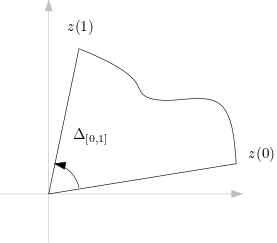
\includegraphics[scale=0.8]{deltaarg.png}
    \caption{Приращение аргумента вдоль кривой}
		\label{fig:14.1}
\end{figure}\\
\theorem (логарифмическое свойство)
Пусть $z(t) \in C^1[0;1]$, $\forall t \in [0,1] z(t) \neq 0$. Пусть $z(t) =
z_1(t)z_2(t)$, $z_k(t) \in C^1[0,1]$. Тогда
\begin{equation}\label{(14.8)}
    \Delta_{[0,1]}\argt z = \Delta_{[0,1]}\argt z_1 + \Delta_{[0,1]}\argt z_2
\end{equation}
\pr
Из \eqref{(14.7)} имеем:
\begin{align*}
  & \Delta_{[0,1]} \argt z(t) = \Img \int_{0}^{1}\frac{\left( z_1(\tau)z_2(\tau) \right)'}{z_1(\tau)z_2(\tau)}d \tau =\Img \int_{0}^{1}\frac{z_1'z_2+z_1z_2'}{z_1z_2}d \tau = \Img \int_{0}^{1}\frac{z_1'}{z_1}d \tau + \Img \int_{0}^{1}\frac{z_2'}{z_2}d \tau = \\
  & = \Delta_{[0,1]} \argt z_1(t) \Delta_{[0,1]} \argt z_2(t) 
\end{align*}
\Def
Пусть $\gamma$~--- кривая в $\CC$, заданная параметризацией $z=z(t)$, $t \in
[0;1]$, $z \in C^1[0;1]$, $0 \not \in \gamma$. Тогда \textbf{приращением
  аргумента $z$ вдоль кривой $\gamma$} называется
\begin{equation}\label{(14.9)}
    \Delta_{\gamma}\argt z = \Delta_{[0;1]}\argt z = \Img \int_{0}^1 \frac{z'(\tau)}{z(\tau)}d \tau
\end{equation}
Определение корректно, т.~к. \eqref{(14.9)} равносильно
\begin{equation}\label{(14.10)}
    \Delta_{\gamma}\argt z = \Img \int_{\gamma} \frac{dz}{z}
\end{equation}
	\begin{flushright}
    \textit{Лекция 11 (от 12.10)}
\end{flushright}
\section{$\S 15.$ Регулярные ветви многозначных функций $\{\sqrt{z}\}$ и $\Ln z$.}

	\begin{flushright}
    \textit{Лекция 12 (от 13.10)}
\end{flushright}
\corollary
Пусть $G$ односвязна, $0 \not \in G$. Тогда для регулярной $h_k \in \Ln z$
справедлива формула Ньютона-Лейбница
\begin{equation}\label{(15.14)}
    h_k(z) = h_k(a) + \int_{\gamma_{az}}\frac{d\zeta}{\zeta}
\end{equation}
где $a \in G$, $\gamma_{az} \subseteq G$.
\pr
\begin{align*}
  & h_k(z) = h_0(z) + 2i \pi k
\end{align*}
\begin{align*}
  & h_0(z) = \ln \left| z \right| + i \left( \psi_0 + \Delta_{\gamma_{az}}\argt z \right)
\end{align*}
\begin{align*}
  & \Real \int_{\gamma_{az}} \frac{d\zeta}{\zeta} = \ln \left| z \right| - \ln \left| a \right|
\end{align*}
Действительно, пусть $z(t) = \gamma_{az}$, тогда
\begin{align*}
  & \Real \int_{\gamma_{az}} \frac{d\zeta}{\zeta} = \Real \int_0^1 \frac{xx'+yy'}{x^2+y^2} d \tau = \Real \int_0^1 \frac{d \sqrt{x^2+y^2}}{\sqrt{x^2+y^2}} = \ln \left| z(1) \right| - \ln \left| z(0) \right| = \ln \left| z \right| - \ln \left| a \right|
\end{align*}
\begin{align*}
  & h_k(z) = \ln \left| z \right| - \ln \left| a \right| + \ln\left| a \right| + i \left( \psi_0 + 2 \pi k \right) + i \Delta_{\gamma_{az}}\argt z = h_k(a) + \int_{\gamma_{az}}\frac{d\zeta}{\zeta}
\end{align*}
\section{$\S 16$. Регулярные ветви $\{\sqrt[n]{f(z)}\}$ и $\ln f(z)$.}
\sug
$G$~--- область, $f$ регулярна на $G$, $\forall z \in G \ f(z) \neq 0$.
\begin{equation}\label{(16.1)}
    \left\{ \sqrt[n]{f(z)} \right\} = \sqrt[n]{\left| f(z) \right|} \exp \left( \frac{i}{n}\Arg f(z) \right)
\end{equation}
\begin{equation}\label{(16.2)}
    \Ln f(z) = \ln \left| f(z) \right| +i \Arg f(z)
\end{equation}
\begin{equation}\label{(16.3)}
    \Arg f(z) = \left\{ \argt f(z) + 2 \pi k \mid k \in \ZZ \right\}
\end{equation}
\Def
Пусть $\gamma$~--- непрерывная кривая в $G$, $f$ удовлетворяет предположению
$1$. Пусть $z(t)$~--- параметризация $\gamma$, $t \in [0;1]$. Пусть $\Gamma =
f(\gamma): \ w = f(z(t)), \ t \in [0;1]$. Тогда \textbf{приращением аргумента
  $f(z)$ вдоль кривой $\gamma$} называется
\begin{equation}\label{(16.4)}
    \Delta_{\gamma}\argt f(z) = \Delta_\Gamma\argt w = \Delta_{[0;1]}\argt f(z(t))
\end{equation}
\lemma
Пусть $f$, $f_1$, $f_2$ удовлетворяют предположению $1$ в области $G$. Тогда
\begin{enumerate}
    \item для любой непрерывной $\gamma \subseteq G$ выполняется логарифмическое
    свойство:
    \begin{equation}\label{(16.5)}
        \Delta_{\gamma}\argt (f_1f_2) = \Delta_\gamma\argt f_1 + \Delta_{\gamma}\argt f_2
    \end{equation}
    \item если $\gamma \subseteq G$ разбита точкой $A \in \gamma$ на части
    $\gamma_1$, $\gamma_2$, то
    \begin{equation}\label{(16.6)}
        \Delta_{\gamma}\argt f = \Delta_{\gamma_1}\argt f + \Delta_{\gamma_2}\argt f
    \end{equation}
    \item если $\gamma$~--- кусочно гладкая кривая в $G$, то
    \begin{equation}\label{(16.7)}
        \Delta_{\gamma}\argt f(z) = \Img \int_\Gamma \frac{dw}{w} = \Img \int_{\gamma} \frac{f'(\zeta)}{f(\zeta)}d\zeta
    \end{equation}
\end{enumerate}
\pr
Утверждения леммы очевидны из определения приращения аргумента функции.
\lemma
Пусть $G$ односвязна, $\os{\circ}{\gamma} \subseteq G$ замкнута и непрерывна.
Пусть $f$ удовлетворяет предположению $1$. Тогда
\begin{equation}\label{(16.8)}
    \Delta_{\os{\circ}{\gamma}}\argt f(z) = 0
\end{equation}
\pr
Пусть $\os {\circ}{\gamma} \subseteq G$ гладкая и замкнутая, параметризованная
$z(t)$.
\\
$\forall z_0 \in \os{\circ}{\gamma}$ существует непрерывная деформация $z(t,
\alpha)$ такая, что $z(t,a) = z(t)$, $z(t,b) = z_0$. По теореме $3$ $\S 14$
$I(\alpha) = const$, а значит,
\begin{align*}
  \Delta_{[0;1]}\argt f(z) = \Delta_{[0;1]}\argt f(z_0) = 0
\end{align*}
\lemma
Пусть $f$ удовлетворяет предположению $1$ в области $G$. Если в области $G$
сществуют регулярные ветви $h_0(z)$ или $g_0(z)$~--- регулярные ветви $\Ln f(z)$
или $\left\{ \sqrt[n]{f(z)} \right\}$, то все их непрерывные ветви регулярны и
удовлетворяют соотношениям:
\begin{equation}\label{(16.9)}
    h_k(z) = h_0(z) + 2i \pi k, \ k \in \ZZ
\end{equation}
\begin{equation}\label{(16.10)}
    g_k(z) = g_0(z) \exp\left( \frac{i}{n} 2 \pi k\right), \ k \in \{0, \dots, n-1\}
\end{equation}
\pr
Доказательство полностью аналогично доказательству леммы $15.1$.
\lemma
Пусть $f$ удовлетворяет предположению $1$ в $G$. Если в $G$ существует
регулярная ветвь $h(z)$ многозначной функции $\Ln z$, то $\forall a,b \in G$
\begin{equation}\label{(16.11)}
    h(b) = h(a) + \ln \left| \frac{f(b)}{f(a)} \right| + i \Delta_{\gamma_{ab}}\argt f(z)
\end{equation}
\pr
\begin{align*}
  & h(z) = \ln \left| f(z) \right| + i \Img h(z)
\end{align*}
В силу регулярности $h$ $\Img h$ будет гармонической функцией от $x, y$. Значит,
\begin{align*}
  & \varphi(z) = \Img h(z) \in \Arg f(z)
\end{align*}
Пусть $a \in G$, $\psi_0 \in \Arg f(a)$, $h(a) = \ln \left| f(a) \right| + i
\psi_0$. Пусть $\gamma_{az}$~--- гладкая кривая с параметризацией $z(t)$, $t \in
[0;1]$, $\varphi(z(t))$~--- гладкая ветвь $\Arg f(z(t))$.
\begin{align*}
  & \Delta_{\gamma_{az}}\argt f(z) = \varphi(z(1))-\varphi(z(0)) = \Img h(z) - \Img h(a)
\end{align*}
\begin{align*}
  & h(b) = \ln \left| f(b) \right| + i \Img h(b)
\end{align*}
\begin{align*}
  & h(a) = \ln \left| f(a) \right| + i \Img h(a)
\end{align*}
\begin{align*}
  & h(b) - h(a) = \ln \left| \frac{f(b)}{f(a)} \right| + i \left( \Img h(b) - \Img h(a) \right)
\end{align*}
Отсюда следует \eqref{(16.11)}.
\theorem
Пусть $f$ удовлетворяет предположению $1$ в $G$. Тогда у  $\Ln f(z)$ существуют
регулярные ветви в $G$ тогда и только тогда, когда выполняется \eqref{(16.8)}
для любой замкнутой $\os{\circ}{\gamma}\subseteq G$.
\pr
Докажем в обе стороны.
\begin{itemize}
    \item Необходимость.
    \\
    Если есть регулярные ветви $h(z) \in \Ln z$  $G$, то из \eqref{(16.11)} при
    $a = b$ получаем \eqref{(16.8)}.
    \item Достаточность.
    \\
    Пусть выполнено \eqref{(16.8)}. Фиксируем $a \in G$, $h(a) \in \Ln f(a)$.
    Рассмотрим
    \begin{equation}\label{(16.12)}
        h(z) = h(a) + \ln \left| \frac{f(z)}{f(a)} \right| + i \Delta_{\gamma_{az}}\argt f(z)
    \end{equation}
    В действительности приращение аргумента может зависеть от $\gamma$, поэтому
    корректнее расссматривать это как $h(\gamma_{az})$.
    \\
    По \eqref{(16.8)}
    \begin{align*}
      & \Delta_{\gamma_{az}}\argt f(z) = \Delta_{\tilde{\gamma}_{az}} f(z)
    \end{align*}
    \begin{align*}
      & \os{\circ}{\gamma} = \gamma_{az}+\tilde{gamma}^{-1}_{az}
    \end{align*}
    Значит, $h(z)$~--- функция лишь точки $z$.
    \begin{equation}\label{(16.13)}
        \exists \psi_0 \in \Arg f(a): \ h(a) = \ln \left| f(a) \right| + i \psi_0
    \end{equation}
    Из \eqref{(16.12)} следует, что
    \begin{align*}
      & h(z) = \ln \left| f(z) \right| + i \left( \psi_0 + \Delta_{\gamma_{az}}\argt f(z) \right) \in \Ln f(z)
    \end{align*}
    \begin{align*}
      & \Real \int_{\gamma_{az}}\frac{f'(\zeta)}{f(\zeta)}d\zeta = \ln \left| f(z) \right| - \ln \left| f(a) \right|
    \end{align*}
    \begin{align*}
      & \Delta_{\gamma_{az}}\argt f(z) = \Img \int_{\gamma_{az}}\frac{f'(\zeta)}{f(\zeta)}d\zeta
    \end{align*}
    Отсюда следует, что
    \begin{align*}
      & h(z) = \ln \left| f(a) \right| + \ln \left| f(z) \right| - \ln \left| f(a) \right| + i \Delta_{\gamma_{az}} \argt f(z) + i \psi_0 = \ln \left| f(a) \right| + \int_{\gamma_{az}}\frac{f'(\zeta)}{f(\zeta)}d \zeta
    \end{align*}
    Функция
    \begin{align*}
      & \varphi(z) = \int_{\gamma_{az}}\frac{f'(\zeta)}{f(\zeta)}d\zeta
    \end{align*}
    регулярна по теореме $3$ $\S 6$, а значит, и $h(z)$ регулярна.
\end{itemize}
\lemma
Пусть $f$ удовлетворяет предположению $1$ в $G$, $n \in \NN$, $n \geq 2$. Если в
$G$ существует регулярная ветвь $g(z)$ многозначной функции $\left\{
    \sqrt[n]{f(z)} \right\}$, то $\forall a, b \in G$
\begin{equation}\label{(16.14)}
    g(b) = g(a) \sqrt[n]{\left| \frac{f(b)}{f(a)} \right|}\exp \left( \frac{1}{n}\Delta_{\gamma_{ab}}\argt f(z) \right)
\end{equation}
\pr Доказательство разбиваем на два этама.
\begin{enumerate}
    \item $G$ односвязна.
    \\
    По лемме $2$ $\forall \os{\circ}{\gamma} \subseteq G$ выполняется
    \eqref{(16.8)}:
    \begin{align*}
      & \exists h(z) = h(a) + \ln \left|\frac{f(z)}{f(a)}\right|+ i\left(\Delta_{\gamma_{az}}\argt f(z)\right) \in \Ln f(z)
    \end{align*}
    регулярные ветви.
    \begin{align*}
      & g_0(z) = \exp \left(\frac{i}{n} h(z)\right)
    \end{align*}
    \begin{align*}
      & \exists \psi_0 \in \Arg f(a): \ h(z) = \ln \left| f(z) \right| + i \left( \psi_0 + \Delta_{\gamma_{az}}\argt f(z) \right)
    \end{align*}
    Тогда
    \begin{align*}
      & g_0(z) = \sqrt[n]{\left| f(z) \right|}\exp \left( \frac{i}{n} \left( \psi_0 + \Delta_{\gamma_{az}}\argt f(z) \right) \right)\in \left\{ \sqrt[n]{f(z)} \right\}
    \end{align*}
    регулярная ветвь.
    \\
    По лемме $3$ $\exists k \in \left\{ 0, \dots, n-1 \right\}: \ g(z) = g_0(z)$.
    Отсюда следует \eqref{(16.14)}.
    \item $G$~--- область.
    \begin{align*}
      &\forall a, b \in G, \ \forall \gamma_{ab} \subseteq G
    \end{align*}
    можем выбрать такие $a=z_0, z_1, \dots, z_{K-1}, z_K = b \in \gamma_{ab}$,
    что $\left| z_k - z_{k-1} \right|< l_k$, где $l_k$~--- расстояние до
    границы.
    \begin{align*}
      & \exists \left\{ B_\varepsilon(z_k) \right\}_{k=0}^K \subseteq G: \ z_{k+1} \in B_{\varepsilon}(z_k)
    \end{align*}
    Каждый из $B_{\varepsilon}(z_k)$ односвязен, поэтому выполняется
    \eqref{(16.14)}:
    \begin{align*}
      & \forall k \in \left\{ 0, \dots, K-1 \right\} \ \frac{g(z_{k+1})}{g(z_k)} = \sqrt[n]{\frac{f(z_{k+1})}{f(z_k)}} \exp \left( \frac{i}{n} \Delta_{\gamma_{z_kz_{k+1}}}\argt f(z) \right)
    \end{align*}
    Перемножая по всем $k$, получаем
    \begin{align*}
      & \frac{g(b)}{g(a)} = \sqrt[n]{\left| \frac{f(b)}{f(a)} \right|}\exp \left( \frac{i}{n} \sum_{k=0}^{K-1} \Delta_{\gamma_{z_kz_{k+1}}} \argt f(z) \right) = \sqrt[n]{\frac{\left| f(b) \right|}{\left| f(a) \right|}}\exp \left( \frac{i}{n}\Delta_{\gamma_{ab}}\argt f(z) \right)
    \end{align*}
    Это ни что иное, как \eqref{(16.14)}.
\end{enumerate}\theorem
Пусть $f$ удовлетворяет условиям предположения $1$ в $G$. Тогда существуют
регуляртые ветви $\left\{ \sqrt[n]{f(z)} \right\}$тогда и только тогда, когда
\begin{equation}\label{(16.15)}
    \forall \os{\circ}{\gamma} \subseteq G \exists k(\os{\circ}{\gamma}) \in \ZZ: \ \Delta_{\os{\circ}{\gamma}}\argt f(z) = 2\pi n k(\os{\circ}{\gamma}))
\end{equation}
\end{document}